% preamble for "jsartcle"

\documentclass[a4paper, dvipdfmx, 9truept, 9trueptj]{jsreport}
\usepackage[top=30truemm,bottom=30truemm,left=25truemm,right=25truemm]{geometry}

\usepackage{amsmath, amssymb, amsthm}
% \usepackage{ascmac}
\usepackage{mathtools}
\mathtoolsset{showonlyrefs=true}
\usepackage{bm}
\usepackage{graphicx}

\usepackage{cancel}
\usepackage{mathrsfs}
\usepackage{algorithm}
\usepackage{algpseudocode}

\usepackage{tikz}
\usetikzlibrary{patterns}



%-------定理環境のカスタマイズ

% \newtheoremstyle{mystyle}%   % スタイル名
%     {3truept}%                   % 上部スペース
%     {3truept}%                   % 下部スペース
%     {\itshape}%              % 本文フォント
%     {9truept}%               % 1行目のインデント量
%     {\bfseries}%             % 見出しフォント
%     {.}%                     % 見出し後の句読点
%     {\\}%                      % 見出し後のスペース
%     {}%                      % 見出しの書式(後述)
\newtheoremstyle{break}
  {\topsep}{\topsep}%
  {}{}%
  {\bfseries}{.}%
  {\newline} {\thmname{#1}\thmnumber{ #2}\thmnote{ \bfseries{(#3)}}}%
% \@addtoreset{theorem}{subsection}
%以下、定理環境の日本語化
\theoremstyle{break}
\newtheorem{theorem}{定理}
% \newtheorem*{theorem*}{定理}
\newtheorem{definition}[theorem]{定義}
% \newtheorem*{definition*}[theorem]{定義}
\newtheorem{lemma}[theorem]{補題}
\newtheorem{corollary}[theorem]{系}
\newtheorem{proposition}[theorem]{命題}% jsarticleのみ
\newtheorem{example}[theorem]{例}
\newtheorem*{example*}{例}
\newtheorem{problem}[theorem]{問題}
\newtheorem{solution}[theorem]{解}
\newtheorem{fact}[theorem]{事実}
\newtheorem{remark}[theorem]{remark}
\newtheorem*{remark*}{remark}
\def\proofname{証明}

%-------番号のカスタマイズ
\numberwithin{equation}{section}
\numberwithin{theorem}{section}

%-------マクロ
\newcommand{\groebner}[1]{Gr\"{o}bner#1}
\newcommand{\ideal}[1]{\langle #1 \rangle}
% \newcommand{\ht}{\mathrm{ht}}
% \newcommand{\hc}{\mathrm{hc}}
% \newcommand{\hm}{\mathrm{hm}}
\renewcommand{\algorithmicrequire}{\textbf{input:}}
\renewcommand{\algorithmicensure}{\textbf{output:}}
\newcommand{\ForTo}[1]{\; \mathbf{to} \; #1}
\newcommand{\ForToBy}[2]{\; \mathbf{to} \; #1 \; \mathbf{by} \; #2}
\newcommand{\ForEach}[1]{\mathbf{each} \; #1}
\algdef{SE}[DOWHILE]{Do}{doWhile}{\algorithmicdo}[1]{\algorithmicwhile\ #1} %do-while文
% ---使用例---
% \Do
% 	\State Something
% \doWhile{$i = j$}
% のように使う






\begin{document}
	% ------title and abstract
	
% \title{パラメータを伴った\groebner{}基底の構造的な検出について}
% \subtitle{SGBD}
% \author{大島谷遼}
% \date{\today}

% ------title
\begin{center}
	{
		\fontsize{15truept}{0truept}\selectfont
		パラメータを伴った\groebner{}基底の構造的な検出について
	}
\end{center}

% ------subtitle
\begin{flushright}
	--- Comprehensive structural \groebner{} basis detection ---
\end{flushright}

% ------other
\begin{minipage}{0.49\columnwidth}
	\phantom{fight!}
\end{minipage}
\begin{minipage}{0.49\columnwidth}
	{
		\fontsize{12truept}{17truept}\selectfont
		\begin{tabular}[htbp]{ll}
			所属専攻 &人間環境学専攻\\
			学籍番号 &208D418D\\
			学\hspace{7.33truept}生\hspace{7.33truept}氏\hspace{7.33truept}名 &大島谷 遼\\
			指導教員氏名 &長坂 耕作  准教授
		\end{tabular}
	}
\end{minipage}
\\

% ------main
本論文では,パラメータを伴った多項式集合$F$がそのまま$\ideal{F}$の\groebner{}基底となっているような項順序を求める方法について論じる.
\par
パラメータを伴っていない多項式集合において,この問題は\groebner{} basis detection(GBD)と呼ばれている.GBDはSturmfelsらにより,affine Newton polyhedronを用いて項順序を同値類に分類し,それぞれの代表元においてS多項式が全て$0$へと簡約される($\Leftrightarrow$ 「\groebner{}基底となっている」)ことを確かめるという方法が提案されている\cite{gritzmann1993minkowski}.しかし,このアルゴリズムでは結局S多項式の簡約化の計算を(多くの場合では)複数回行わなくてはならず,与えられたアルゴリズムはNP-Hardであることが分かっている\cite[Corollary11]{sturmfels1997structural}.そこで,問題の条件を,「先頭項同士が全て互いに素となるような項順序は存在するか」(Buchbergerの判定条件)という\groebner{}基底となるための十分条件に置き換えて問題を簡単にする.この問題をstructural \groebner{} basis detection(SGBD)と呼ぶ.SGBDについても,Sturmfelsらによって二部グラフの最大マッチング問題と線形計画問題に帰着されたアルゴリズムが存在しており,多項式集合の濃度を固定したときにはNP-Compreteであることが証明されている\cite[Corollary3]{sturmfels1997structural}.
\par
本論文では,特にこのSGBDに着目し,多項式集合がパラメータを伴った場合についての拡張を行う.パラメータを伴ったSGBDは,最初にパラメータ空間を包括的に分割することで,後に新たな場合分けを発生させずに通常のSGBDのアルゴリズムを計算することができる.また,このような直接的な方法の他にも,affine Newton polyhedronや,多項式環の加群の包括的\groebner{}基底系を用いてパラメータを伴ったSGBDを効率化する方法についても議論している.









	\phantom{fight!}\par

計算機代数の分野において重要な計算の$1$つに\groebner{}基底の計算がある.
\groebner{}基底の計算はBuchbergerアルゴリズム\cite{buchberger2006bruno}に代表されるように,イデアルと項順序を指定して,一定の条件を満たすようなイデアルの基底を求めるものである.
$F_4$アルゴリズム\cite{faugere1999new}など他の多くのアルゴリズムでも,Buchbergerアルゴリズムの系譜が受け継がれており,基本的なアルゴリズムの考え方は変わっていない.
\par
一方で,以下の例のように,与えられた多項式集合$F$がある項順序においてそのままイデアル$\ideal{F}$の\groebner{}基底となっているような場合が存在する.
\begin{example*}
	以下の多項式集合$F$は,$z \succ y \succ x$の全次数辞書式順序及び全次数逆辞書式順序においてイデアル$I = \ideal{F}$の\groebner{}基底となっている.
	$$F = \left\{ 2xy + yz, \; x^2 + y + z \right\} \subset \mathbb{C}[x, y, z]$$
\end{example*}
このように,直接\groebner{}基底の計算をする前に,計算対象である$F$自身がそのまま\groebner{}基底となっているような項順序を求めることができれば,項順序を指定しない\groebner{}基底が必要な場面では有効な計算方法であることが考えられる.また,仮に一定の項順序が必要な場面でも,FGLMアルゴリズム\cite{faugere1993efficient}や\groebner{} walk\cite{collart1993grobner}などに代表されるchange of orderingのアルゴリズムを活用することによって,有用な計算手段となることが考えられる.
\par
例えば,連立代数方程式の求解のための計算では,多くの場合で辞書式順序(一般的には消去順序)での\groebner{}基底が必要となるが,辞書式順序での計算は遅くなることが知られており,入力の多項式集合の大きさによっては
\par
このように「そのまま\groebner{}基底である」ような項順序を検出する問題は,Sturmfelsらによって解かれた既知の問題であり,\emph{\groebner{} basis detection}\cite{gritzmann1993minkowski}や\emph{Structural \groebner{} basis detection}\cite{sturmfels1997structural}という名前が付けられている.
本論文では,これらの問題において,問題の設定をパラメータを伴った多項式環へと拡張し,それに付随して発見された定理についても取り上げる.
まず第\ref{chapter01:chapter_num}章では,Sturmfelsらとは違ったアプローチから,\emph{Structural \groebner{} basis detection}の問題を捉え,そこで新たに発見された定理を紹介する.
次に,第\ref{chapter02:chapter_num}章では,\emph{\groebner{} basis detection}と\emph{Structural \groebner{} basis detection}について,既に知られている部分について述べる.
第\ref{chapter03:chapter_num}章では,これらの問題をパラメータを伴った多項式環へと拡張するために,パラメータ空間を分割するためのアルゴリズムの直接的な方法を紹介する.
最後に,第\ref{chapter04:chapter_num}章では,パラメータ空間の分割を効率化するための議論を行い,最終的なアルゴリズムを完成させる.


	\tableofcontents

	% ------chapter01
	\chapter{はじめに}\label{chapter01:chapter_num}
	% \chapter{はじめに}
\section{研究の背景}
多項式集合$F$が与えられイデアル$\ideal{F}$での\groebner{}基底の計算を行う際,Buchbergerアルゴリズム\cite{buchberger2006bruno}などにより項順序を固定した上で,\groebner{}基底を得るための計算を行うのが一般的である.
しかし,以下の例のように,計算を行う前に$F$がそのまま\groebner{}基底であるような項順序を得ることができる場合もある.
\begin{example}
	以下の多項式集合$F$は,$z \succ y \succ x$の全次数辞書式順序及び全次数逆辞書式順序においてイデアル$I = \ideal{F}$の\groebner{}基底となっている.
	$$F = \left\{ 2xy + yz, \; x^2 + y + z \right\} \subset \mathbb{C}[x, y, z]$$
\end{example}
このような項順序を見つけることができれば,従来の計算を行わずに\groebner{}基底を得ることができる.
また,ここで得た項順序を,FGLMアルゴリズム\cite{faugere1993efficient}や\groebner{} walk\cite{collart1993grobner}などに代表されるchange of orderingのアルゴリズムによって変換することで,任意の項順序での\groebner{}基底を得ることも可能であり,有効な計算手段となることが考えられる.
\par
例えば,多変数の連立代数方程式の解を求めるためには,多くの場合で辞書式順序(一般的には消去順序)での\groebner{}基底が必要となるが,辞書式順序での計算は遅くなることが知られており,入力の多項式集合の大きさによっては莫大な時間がかかってしまう可能性も否定できない.そこで,多項式集合がそのまま\groebner{}基底となっているような項順序が存在していれば,その項順序を求めたあとにchange of orderingにより辞書式順序の\groebner{}基底を求めることができる.これらの$2$つの計算の計算量が,元々行おうとしていた\groebner{}基底計算の計算量に比べて少なくなっているのであれば,この計算は有用な計算であったと言える.
\par
このように「そのまま\groebner{}基底である」ような項順序を検出する問題は,\emph{\groebner{} basis detection}\cite{gritzmann1993minkowski}や\emph{structural \groebner{} basis detection}\cite{sturmfels1997structural}という名前が付けられており,何れもSturmfelsらによって解かれた既知の問題である.
\par
一方で,パラメータを伴った多項式環において,場合分けされたパラメータ空間と,それぞれに対応する\groebner{}基底を組にしたものを\textbf{包括的\groebner{}基底系}\cite{weispfenning1992comprehensive}と呼ぶ.包括的\groebner{}基底系は,\groebner{}基底計算の中で,\textrm{S-polynomial}の計算が行われる際にパラメータの付いた係数が$0$か否かで場合分けを行い,項を確定させながら\groebner{}基底の計算を行われているが,現在はより効率的な方法が考案されている\cite{kapur2010new}.
\par
これら$2$つの議論を踏まえ,本論文では,(structural) \groebner{} basis detectionにおいて,問題の設定をパラメータを伴った多項式環へと拡張し,それに付随して発見された定理についても取り上げる.
まず第\ref{chapter02:chapter_num}章では,Sturmfelsらとは違ったアプローチでstructural \groebner{} basis detectionの問題を捉え,そこで新たに発見された定理とアルゴリズムを紹介する.
次に,第\ref{chapter03:chapter_num}章では,\groebner{} basis detectionとstructural \groebner{} basis detectionについて,既に知られている部分について述べる.
第\ref{chapter04:chapter_num}章では,これらの問題をパラメータを伴った多項式環へと拡張するために,パラメータ空間を分割するためのアルゴリズムの直接的な方法と,分割の効率化のための方法について記す.% 研究の背景
	% chapter01_はじめに
\section{基本的な定義}
以下では本論文全体を通して使用される記法を定義しておく.
\par
$\mathbb{N}$は$0$以上の整数全体の集合とする.$K$を体とし,$L$を$K$の代数閉包とする.
$n$個の変数全体の集合を$\bar{X} = \{x_1, \dots, x_n\}$とし,$m$個のパラメータ全体の集合を$\bar{A} = \{a_1, \dots, a_m\}$とする.ただし,$\bar{X}\cap \bar{A} = \phi$.$T(f)$を$f$の$0$でない項全体の集合とする.
$n$変数の項全体の集合を$T_n = \left\{ x_1^{e_1} \cdots x_n^{e_n} : e_i \in \mathbb{N} \right\}$とする.
項順序を次のように定義する.
\begin{definition}[項順序]
	$T_n$における全順序$\prec$が項順序であるとは,
	\begin{itemize}
		\item 任意の$t \in T_n$に対し$1 \prec t$
		\item 任意の$t_1, t_2, s \in T_n$に対し,$t_1 \prec t_2 \Longrightarrow s\cdot t_1 \prec s\cdot t_2$
	\end{itemize}
	を満たすことを言う.
\end{definition}
項順序$\prec$において,多項式$f\in K[\bar{X}]$に含まれる項で,最も項順序が大きい単項式を$\mathrm{hm}_{\prec}(f)$,その係数を除いた部分を$\mathrm{ht}_{\prec}(f)$,その係数を$\mathrm{hc}_{\prec}(f)$と定義し,それぞれ\textbf{頭単項式,頭項,頭係数}と呼ぶ.
項順序が明らかな場合には,$\mathrm{hm}_{\prec}(f)$を単に$\mathrm{hm}(f)$などと書くこともある.
また,多項式集合$F$に関して,$\mathrm{HM}_{\prec}(F) = \{ \mathrm{HM}_{\prec}(f_i) \;:\; f_i \in F \}$と定義する($\mathrm{HT}_{\prec}(F), \mathrm{HC}_{\prec}(F)$についても同様に定義する).
項$t \in T_n$の指数ベクトルを$e(t) \in \mathbb{N}^{n}$と表す.
重み行列$M$で表されるmatrix order$\prec_M$を以下のように定義する.
\begin{definition}[matrix order]
	項$t_1, t_2 \in T_n$の指数ベクトル$e(t_1), e(t_2) \in \mathbb{N}^{n}$に対し,行列$M \in \mathbb{R}^{d\times n}$がmatrix orderであるとは,
	$$t_1 \prec_M t_2 \Longleftrightarrow Me(t_1) <_{\ne} Me(t_2)$$
	を満たすことを言う.ただし,$<_{\ne}$や$>_{\ne}$は,ベクトルの等しくない最初の成分での比較を表す不等号である.$d=1$のときは,通常の大小関係での比較となる.
\end{definition}
matrix orderは任意の項順序を表現可能である\cite{MR826583}ということがわかっており,column full rankな行列を考えれば十分であるということもわかっている.
\par
項順序を$M$とする.多項式$f, g \in K[\bar{X}]$に対し,$f$に含まれる単項式$t$が$\mathrm{ht}_M(g)$で割り切られるとする.このとき,$h = f - \frac{t}{\mathrm{ht}_M(g)}g$に対し,$f \to_g h$と書き,\textbf{$f$の$g$での単項簡約}と呼ぶ.この操作を$0$回を含む有限回繰り返し,これ以上単項簡約できない$h$が得られたとき,$h$を\textbf{$f$の$g$による正規形(normal form)}と呼び,$h = \mathrm{nf}_g(f)$で表す.
また,有限な多項式集合$G=\left\{g_i :i \in \{1,2, \dots\}\right\} \subset K[\bar{X}]$において,$g_i \in G$で$f$を単項簡約することを繰り返すことで$h$が得られるとき,同様に$h$を\textbf{$f$の$G$による正規形}と呼び,$h = \mathrm{nf}_G(f)$で表す.
\begin{definition}[S多項式]
	項順序を$M$とし$f, g \in K[\bar{X}]$とする.このとき,$f, g$のS多項式を次のように定義する.
	$$\mathrm{Spoly}(f, g)=\frac{\mathrm{hc}_M(g)\cdot \mathrm{lcm}(\mathrm{ht}_M(f), \mathrm{ht}_M(g))}{\mathrm{ht}_M(f)}\cdot f - \frac{\mathrm{hc}_M(f)\cdot \mathrm{lcm}(\mathrm{ht}_M(f), \mathrm{ht}_M(g))}{\mathrm{ht}_M(g)}\cdot g$$
	\end{definition}








% 基本的な定義
	
	% ------chapter02
	\chapter{項順序についての再考}\label{chapter02:chapter_num}
	% chapter 02
\section{はじめに}
この章では,後に紹介するstructural \groebner{} basis detectionと同じ問題設定において,Sturmfelsらによる方法とは違った独自のアプローチによるアルゴリズムを考案する中で発見した新たな定理やアルゴリズムについて述べる.第\ref{chapter01:chapter_num}章にあったとおり,項順序$M$はcolumn full rankな行列を考えれば,項順序を十分に定義できることが分かっているため,この章では$M$を$n \times n$の正方で正則な行列であると仮定する.ただし,$n$は主変数の個数である.
\par
目標とする問題は次の通りであった.
\begin{problem}
	\label{chapter02:problem:original_SGBD}
	多項式集合$F$がイデアル$I = \ideal{F}$の\groebner{}基底となるような項順序$M$を求めよ.
\end{problem}
この問題を解くにあたって,\groebner{}基底となるための必要十分条件ではなく,以下の定理\ref{chapter02:theorem:buchbergers_criterion}をもとに十分条件を考えることで,系\ref{chapter02:corollary:buchberger}を満たすような項順序$M$を考える(この問題は,後に説明するstructural \groebner{} basis detectionと同じ問題設定である).
\begin{theorem}[Buchbergerの判定条件]
	\label{chapter02:theorem:buchbergers_criterion}
	項順序を$M$とする.任意の多項式$f, g \in K[\bar{X}]$において,$$\gcd(\mathrm{ht}_M(f), \mathrm{ht}_M(g))=1$$が成り立つとき,$\mathrm{nf}_{\{f, g\}}(\mathrm{Spoly}(f, g)) = 0$が成立する.
	\end{theorem}
	\begin{corollary}
	\label{chapter02:corollary:buchberger}
	項順序を$M$とする.多項式集合$F=\{ f_1, \dots, f_k \} \subset K[\bar{X}]$に対して,イデアル$I = \ideal{F}$とおく.このとき,
	$$\forall i, j \; (i \ne j), \; \gcd(\mathrm{ht}_M(f_i), \mathrm{ht}_M(f_j))=1$$
	が成り立つとき, $F$は項順序$M$に関する$I$の\groebner{}基底である.
\end{corollary}
つまり,ある項順序において各多項式の頭項同士が全て互いに素であれば,入力の多項式集合はそのまま\groebner{}基底である.
これにより,多項式集合$F = \{f_1, \dots, f_k\}\subset K[\bar{X}]$に対して問題\ref{chapter02:problem:original_SGBD}を解くためには次の2つのステップが必要となることがわかる.
\par
\begin{enumerate}
	\item 互いに素な単項式の組$t_1, \dots, t_k$をそれぞれの多項式から選出する.
	\item $i \in \{1, \dots, k\}$において,$\mathrm{ht}_M(f_i) = t_i$となるような項順序$M$を求める.
\end{enumerate}




% はじめに
	% chapter 02
\section{互いに素な項の選出(Step1)}
% 多項式集合$F = \{f_1, \dots, f_k\}\subset K[\bar{X}]$に対して,
% 多項式$f_i$に含まれる係数が$0$でない項で,定数項を除く項全体の集合を$T(f_i)$とする.
% また多項式集合$F$に対しても
% $\displaystyle T(F) = \bigotimes_{i=1}^k T(f_i)$と定義する.
集合$V(t)$を項$t$に含まれる次数$1$以上の変数全体の集合とし,集合$T_{\mathrm{cp}}$を
$$
T_{\mathrm{cp}} = \{ (t_1, \dots, t_k)\in T(F) \;:\; \forall t_i, t_j \in T_n, \; \gcd(t_i,  t_j)=1\; (i\ne j) \}
$$
とする.
\par
Step1では,互いに素である項を探索し集合$T_{\mathrm{cp}}$を構成したいが,このままでは全探索によってそれぞれが互いに素かどうかのチェックが行う必要が出てしまう.
% そこで,系\ref{chapter02:corollary:buchberger}に関連する性質(確実に互いに素とならない項など)についてのいくつかの補題を与える.
そこで,あらかじめ除外できることが分かっている項は除外しておき,探索のコストをできるだけ小さくしておきたい.
項が除外できる理由として,次の$3$つを考える.
\begin{itemize}
	\item 互いに素となり得ない.
	\item 互いに素にはなるが,それぞれが頭項となるような項順序に矛盾が生じてしまう.
	\item 互いに素にはなるが,同じ多項式内で頭項としたときに矛盾が生じてしまう.
\end{itemize}
\subsection{互いに素となり得ない項の性質}
まず,確実に互いに素とならない場合や,そもそも問題\ref{chapter02:problem:original_SGBD}の解が存在しない場合について考える.
\begin{lemma}
	\label{chapter02:lemma:1}
	多項式集合$F=\{ f_1, \dots, f_k \} \subset K[\bar{X}]\setminus K$において,
	$$f_i \in F, \; t_i \in T(f_i), \; |V(t_i)| > n - k + 1$$
	が成り立つとき,$T_{\mathrm{cp}}$の元で$i$番目の要素が$t_i$であるようなものは存在しない.
\end{lemma}
\begin{proof}
	$|V(t_i)| > n - k + 1$が成り立ち,$T_{\mathrm{cp}}$の元で$i$番目の要素が$t_i$であるようなものが存在すると仮定する.
	定義より,任意の項$t$に対して$|V(t)| \ge 1$が成り立つ.
	従って,$j = 1, \dots, i-1, i+1, \dots, k$において,
	$$t_j \in T(f_j), \quad \sum_j |V(t_j)| \ge k -1$$
	よって,
	\begin{align*}
		|V(t_i)| + \sum_j|V(t_j)| &> (n - k + 1) + (k - 1)\\
		& > n
	\end{align*}
	これより変数の個数の合計が$n$個以上であり$t_1, \dots, t_k$の中に,ある特定の変数を含む項が$2$つ以上存在する.しかし,$T_{\mathrm{cp}}$の定義より,$t_1,\dots, t_k$は互いに素でなくてはならない.\\
	よって,補題\ref{chapter02:lemma:1}が成り立つ.
\end{proof}
\begin{corollary}
	\label{chapter02:cororally:2}
	多項式集合$F=\{ f_1, \dots, f_k \} \subset K[\bar{X}]\setminus K$において次が成り立つ.
	$$n<k \Longrightarrow T_{\mathrm{cp}}= \phi$$
\end{corollary}
系\ref{chapter02:cororally:2}より,$n<k$のときに系\ref{chapter02:corollary:buchberger}を満たすような項順序は存在せず,問題\ref{chapter02:problem:original_SGBD}の解が存在しないことがわかり,補題\ref{chapter02:lemma:1}より,$F$の多項式に含まれる項から互いに素になり得ないものを除外することができる.
\subsection{互いに素にはなるが,矛盾が発生する項の性質}
\subsubsection{互いに素にはなるが,同じ多項式内で頭項としたときに矛盾が生じる項の性質}
\begin{lemma}
	\label{chapter02:lemma:3}
	多項式$f$において,$t \mid t^\prime\; (t \ne t^\prime)$を満たすような項$t, t^\prime \in T(f)$が存在するとき,$t$は$f$の頭項となり得ない.
\end{lemma}
\begin{proof}
	$t \mid t^\prime$より,$t^\prime = rt$と置ける.ただし,$r\in T_n$.
	$t$が$f$の頭項であると仮定する.
	このとき,$t^\prime \prec t$であるため,$rt^\prime \prec rt = t^\prime$となり,項順序の定義に矛盾する.よって,$t$は$f$の頭項となり得ない.
\end{proof}

\subsubsection{互いに素にはなるが,それぞれが頭項となるような項順序に矛盾が生じる項の性質}
\begin{lemma}
	\label{chapter02:lemma:4}
	多項式$f_1, f_2 \in K[\bar{X}]$と単項式$t_1, t_1^\prime \in T(f_1), \; t_2, t_2^\prime \in T(f_2)$に対して,
	$$t_2 \mid t_1^\prime, \; t_1 \mid t_2^\prime$$
	が満たされるとき,$t_1, t_2$はそれぞれの多項式で同時に頭項となり得ない.
	ただし,$t_1 \ne t_1^\prime, t_2 \ne t_2^\prime$.
\end{lemma}
\begin{proof}
	$t_1, t_2$はそれぞれ$f_1, f_2$の頭項であると仮定する.
	仮定より,$t_2 \mid t_1^\prime, \; t_1 \mid t_2^\prime$.
	つまり,
	\begin{align*}
		t_1^\prime &= r_2t_2, \\
		t_2^\prime &= r_1t_1
	\end{align*}
	ただし,$r_1, r_2 \in T_n$.
	いま,$t_2 \succ t_2^\prime$より,
	\begin{align*}
		r_2t_2 & \succ r_2t_2^\prime \\
		t_1^\prime & \succ r_2t_2^\prime & (\because t_1^\prime = r_2 t_2) \\
		t_1 & \succ r_2 \cdot r_1t_1 & (\because t_2^\prime = r_1t_1)
	\end{align*}
	これは,$t_1$が$f_1$の頭項であることに矛盾する.
\end{proof}
\begin{lemma}
\label{chapter02:lemma:5}
	多項式$f_1, f_2 \in K[\bar{X}]$と項$t_1^\prime \in T(f_1), t_2 \in T(f_2)$に対して,
	$$t_2 \mid t_1^\prime$$
	が成り立ち,
	項$t_1 \in T(f_1), t_2^\prime \in T(\frac{t_1^\prime}{t_2}f_2)$に対して,
	$$t_1 \mid t_2^\prime$$
	が成り立つとき,$t_1, t_2$はそれぞれの多項式で同時に頭項になり得ない.
	ただし,$t_1 \ne t_1^\prime, t_2 \ne t_2^\prime$.
\end{lemma}
\begin{proof}
	補題\ref{chapter02:lemma:4}とほぼ同じ手順で証明できる.
\end{proof}

\subsection{アルゴリズムの詳細と具体例}
以上より,まず補題\ref{chapter02:lemma:1}と系\ref{chapter02:cororally:2}によって,互いに素となり得ない項を除外でき,補題\ref{chapter02:lemma:3}によって,同じ多項式内にて頭項としたときに矛盾する項を除外できる.更に,補題\ref{chapter02:lemma:4}と補題\ref{chapter02:lemma:5}によって,複数の多項式間で矛盾が発生する項を除外することにより,探索対象の単項を減らすことができる.これらの性質を用いても,総当たりであることには変わらないが,ひとまずこの性質のみで話を進めることにする.
\par
アルゴリズムは以下のように記述できる.
\begin{algorithm}
	\label{chapter02:algorithm:1}
	\caption{そのままグレブナー基底となっているような項順序の導出}
	\begin{algorithmic}[1]
		\Require 多項式集合$F=\{f_1, \dots, f_k \} \subset K[\bar{X}]$
		\Ensure $F$がイデアル$I = \langle F \rangle$のグレブナー基底であるような項順序$M$又はNone
		\If{$n<k$}:
			\State \Return None
		\EndIf
		\State 補題\ref{chapter02:lemma:1},系\ref{chapter02:cororally:2},補題\ref{chapter02:lemma:3}の条件を満たす$f_i$の項を除外し,新たに$\tilde{F} = \{ \tilde{f_1}, \dots, \tilde{f_k} \}$とする.
		\State $T_{\tilde{F}} \leftarrow T(\tilde{F})$
		\State 補題\ref{chapter02:lemma:4},補題\ref{chapter02:lemma:5}の条件を満たす項の組を含むものを$T_{\tilde{F}}$の中から除外し,$\tilde{T}_{\tilde{F}}$とする.
		\State $T_{\mathrm{cp}}$と$\tilde{T}_{\tilde{F}}$の共通部分を取り,それらを$t_1, \dots, t_k$とする.
		\State $i = 1, \dots , k$において,$\mathrm{ht}_M(f_i)=t_i$となる項順序$M$を求める.
		\State \Return $M$
	\end{algorithmic}
\end{algorithm}

このアルゴリズムをもとに,以下のような例を考えてステップ1の項の除去を実際に行ってみる.
\begin{example}
	次のような多項式集合$F \subset K[x, y]$を考える.
	\begin{equation}
		F = 
		\left\{
		\begin{array}{l}
			f_1 = x^2 + xy + y, \\
			f_2 = x + y^2 \notag
		\end{array}
		\right\}
	\end{equation}
	まず,$f_1$において$y \mid xy$が満たされることから,補題\ref{chapter02:lemma:3}より$xy$が除外される.
	次に,$y \in T(f_1)$と$y^2 \in T(f_2)$において,$y \mid y^2$を満たし,$x \in T(f_2)$と$x^2 \in T(f_1)$において,$x \mid x^2$を満たすことから,補題\ref{chapter02:lemma:4}より$f_1$の$y$と$f_2$の$x$が除外される.
	よって,最終的に
	\begin{equation}
		T(\tilde{F}) = \{ (x^2, y^2) \} \notag
	\end{equation}
	から互いに素となる項の組を選べば良いことになり,
	$$t_1 = x^2, \; t_2 = y^2$$
	となる.
\end{example}

\begin{example}
	次のような多項式集合$F\subset K[x, y, z]$を考える.
	\begin{equation}
		F = 
		\left\{
		\begin{array}{l}
			f_1 = xy + yz, \\
			f_2 = x^2 + y + z \notag
		\end{array}
		\right\}
	\end{equation}
	まず,$z \in T(f_2)$と$yz \in T(f_1)$において,$z \mid yz$を満たす.一方で,$f_2$の項を割り切るような$f_1$の項は存在しない.しかし,$yz \div z$の商である$y$を$f_2$に掛け,
	\begin{equation}
		\begin{array}{rl}
			f_1 &= xy + yz, \\
			y\cdot f_2 &= x^2y + y^2 + yz \notag
		\end{array}
	\end{equation}
	を考えると,$xy \in T(f_1)$と$x^2y \in T(y \cdot f_2)$が$xy \mid x^2y$を満たすので,補題\ref{chapter02:lemma:5}より,$f_1$の$xy$と$f_2$の$z$は除外され,最終的に
	\begin{equation}
		T(\tilde{F}) = \{ (yz, x^2), (yz, y) \} \notag
	\end{equation}
	から互いに素となる項の組を選べば良いことになり,
	$$t_1 = yz, \; t_2 = x^2$$
	となる.
\end{example}



















% 互いに素な項の選出(Step1)
	% chpter 02
\section{重み行列$M$の導出(Step2)}
求めたい重み行列$M$を,
$$
	M = \begin{pmatrix}
		\bm{m_1} \\
		\vdots \\
		\bm{m_n}
	\end{pmatrix}
	=
	\begin{pmatrix}
		m_{11} & \cdots & m_{1n} \\
		\vdots & \ddots & \vdots \\
		m_{n1} & \cdots & m_{nn}
	\end{pmatrix}
$$
とする.
matrix orderの定義より,重み行列$M$で表される項順序$\prec$において,項$t_1, t_2$が$t_1 \succ t_2$を満たすとき,$Me(t_1) >_{\ne} Me(t_2)$が満たされる.これを一般の等号と不等号を用いて表すと以下のようになる.
\begin{equation}
	\left\{
	\begin{aligned}
		\bm{m_1} \cdot e(t_1) &= \bm{m_1} \cdot e(t_2)\\
		&\;\; \vdots \\
		\bm{m_{\ell-1}} \cdot e(t_1) &= \bm{m_{\ell-1}} \cdot e(t_2)
	\end{aligned}
	\right.
	\quad
	,
	\quad \bm{m_{\ell}} \cdot e(t_1)> \bm{m_{\ell}} \cdot e(t_2) \notag
\end{equation}
ここで,$\ell$は,$M$の第$(\ell-1)$行ベクトルまでとの積が等しく,第$\ell$ベクトルで初めて差がつくときことを表している.
この連立不等式を解くことによって,重み行列$M$を求めることができるが,その効率的な方法については検討中である.% 項順序Mの導出(Step2)

	% ------chapter03
	\chapter{\groebner{}基底の検出(先行研究の紹介)}\label{chapter03:chapter_num}
	% chapter 03
\section{はじめに}
第\ref{chapter02:chapter_num}章では,項順序をmatrix orderの重み行列$M$で表現し,$M$は多項式環の変数の個数$n$に対して$n$次の正方且つ正則な行列として扱っていた.本章以降は,項順序を重みベクトル$\bm{w}\in \mathbb{R}^n_{+}$にて表現する.ただし,$\mathbb{R}_{+}$は正の実数全体の集合とする.
\begin{remark*}[ベクトルで表現された項順序について]
	項順序はcolumn full rankな行列$M$だけでなくベクトル$\bm{w}\in \mathbb{R}^n_{+}$でも表現可能である.
	ただし,$\bm{w} = (w_i\;:\; i\in \{1, 2, \dots, n\})$において,少なくとも$(n-1)$個の要素が無理数である必要がある.仮に$\bm{w}$に有理数の要素が$2$つ以上存在してしまうと,$\bm{w}$が$\mathbb{Z}$上一次従属となってしまい,項順序の定義である「相異なる項$t_1, t_2 \in T_n$に対して$t_1 \ne_{\bm{w}} t_2$」を満たすことができなくなってしまうためである.
	% \par
	% ベクトル$\bm{w}$に有理数である要素が$w_1,w_2$の$2$つ存在していると仮定すると,
\end{remark*}
\par
この章では,問題\ref{chapter02:problem:original_SGBD}についてのSturmfelsらによる先行研究について述べる.第\ref{chapter02:chapter_num}章では同じ問題設定の中で,互いに素な項の選出を,探索数を減らせるとはいえ全探索により行ったり,求めたい項順序の計算についての効率的な計算方法については与えなかったが,先行研究では,何れにおいても効率的なアルゴリズムが与えられている.
\par
先行研究では,この問題を\emph{\groebner{} basis detection}と名付けており,次のように定義されている.
\begin{definition}[\groebner{} basis detection(GBD)\cite{gritzmann1993minkowski}]
	多項式集合$F \subset K[\bar{X}]$とイデアル$I = \ideal{F}$が与えられたとき,$F$が$I$の\groebner{}基底となるような項順序$\bm{w} \in \mathbb{R}^n_{+}$は存在するか.存在するならば$1$つ求めよ.
\end{definition}
また,GBDの問題をBuchbergerの判定条件(定理\ref{chapter02:theorem:buchbergers_criterion})により簡単にしたものが,次の\emph{structural \groebner{} basis detection}である.
\begin{definition}[structural \groebner{} basis detection(SGBD)\cite{sturmfels1997structural}]
	多項式集合$F \subset K[\bar{X}]$とイデアル$I = \ideal{F}$が与えられたとき,$\mathrm{HT}_{\bm{w}}(F)$に含まれる全ての項が互いに素であるような項順序$\bm{w} \in \mathbb{R}^n_{+}$は存在するか.存在するならば$1$つ求めよ.
\end{definition}











% はじめに
	% chapter 03
\section{\groebner{} basis detection\cite{gritzmann1993minkowski}}
\groebner{} basis detectionの問題を解くあたって,多項式集合の項順序に幾何的な解釈を与えることで,項順序の同値類に分けて考えることができるようになる.ここで,項順序$\bm{w_1}, \bm{w_2}$は,$\mathrm{HT}_{\bm{w_1}}(F) = \mathrm{HT}_{\bm{w_2}}(F)$を満たすときに$F$に関して同値であるという.まずは前提とする定義を与える.
\subsection{前提とする定義}

\begin{definition}[{\cite[p8,9, Definition3.1]{freeke2009linking}}]
	集合$\mathcal{U, V} \subseteq \mathbb{R}^d$に対して,
	\begin{itemize}
		\item $\mathcal{U}$が\textbf{凸(convex)}であるとは,$$\forall \bm{u, v} \in \mathcal{U}, \; \lambda \in \mathbb{R}, \; 0 \le \lambda \le 1, \; \lambda\bm{u} + (1 - \lambda) \bm{v} \in \mathcal{U}$$を満たすときをいう.
		\item \textbf{凸多面体(convex polyhedron)}とは,有限個の半空間の共通部分として得られる凸型の集合である.
		\item 集合$\mathcal{V}$の\textbf{凸包(convex hull)}とは,その集合を含む$\mathbb{R}^d$のすべての凸部分集合の共通部分と定義される.
		\item  $\mathcal{U}$は有界な多面体である場合,\textbf{超多面体(polytope)}と呼ばれる.すべてのpolytopeは,有限の点の集合のconvex hullである.
		% また,polytope $P \subset \mathbb{R}^n$の$\mathcal{V}$-presentationとは,$d$個の点$v_1, \dots, v_d$によって$P = \mathrm{conv} \{v_1, \dots, v_d\}$と表されるときをいう.ただし,$1 \le n < d$.
		% \item 凸多面体$P$の\emph{面(face)}とは,$P$とそれに接する任意の超平面との交点である.$P$のすべての面は,$\mathbb{R}^d$の任意のベクトル$\bm{c}$に対して$\mathrm{face}_c(P) = \left\{ \bm{x} \in P \; : \; \bm{cx} \ge \bm{cy}, \; \forall \bm{y} \in P \right\}$の部分集合である.
		% \item 多面体$P$の面$F$の\emph{次元(demension)}は$\bm{v} \in F$としたときに$\mathbb{R}^d$の部分空間$\bm{v} + H$の次元として定義される.また,$H$はベクトル$\bm{u} \in F, \; \bm{u - v}$によってspanされ,$\bm{v} + H$を$F$の\emph{affine span}と呼ぶ.
		% \item $d$-次元polytopeの$(d - 1)$-次元面を\emph{切子面(facets)}と呼ぶ.
		\item $\mathbb{R}^d$の凸多面体(convex polyhedron)の\textbf{円錐(cone)}$C$は,$$\forall \bm{u, v} \in C, \; \lambda \in \mathbb{R}_{\ge 0}, \; \bm{u+v}, \lambda\bm{u} \in c$$のように定義される.
	\end{itemize}
\end{definition}
$2$つ以上のpolytopeの和を次のように定義する.
\begin{definition}[Minkowski和, {\cite[p247]{gritzmann1993minkowski}}]
	$2$つのpolytope $P_1, P_2 \subset \mathbb{R}^n$に対して,\textbf{Minkowski和}$P_1 + P_2$を
	$$P_1 + P_2 = \{ x \in \mathbb{R}^n \;:\; \exists x_1 \in P_1, \exists x_2 \in P_2, x = x_1 + x_2\}$$
	のように定義する.
	Minkowski和は,可換であり結合法則が成り立つため,$2$つ以上のpolytopeにも自然に一般化することができる.
\end{definition}
% 変数の集合$\bar{X}$に対し,$\bar{X}$の任意の指数ベクトル$\alpha \in \mathbb{N}^n$とし,$K[\bar{X}]$の任意の単項式を$X^\alpha$と表現する.
変数全体の集合$\bar{X} = \{x_1, \dots, x_n\}$に対し,ベクトル$\alpha = (\alpha_i)$で項が$x_1^{\alpha_1} \cdots x_n^{\alpha_n}$と表されるとき,その項を単に$X^{\alpha}$と表す.
また,ベクトル$\bm{u}, \bm{v}$の内積を$(\bm{u}, \bm{v})$と表す.集合$\mathbb{R}_{-}$は$0$以下の実数全体の集合である.
\begin{definition}[Newton polytope]
	多項式$\displaystyle f = \sum_{i=1}^t c_i X^{\alpha_i}$の\textbf{Newton polytope} $\mathcal{N}(f)$を,$\mathbb{R}^n$における単項式のconvex hullで定義する.つまり,
	$$\mathcal{N}(f) = \mathrm{conv}\{\alpha_1, \dots, \alpha_t\}$$
	である.
	また,多項式集合$F = \{f_1, \dots, f_k\} \subset K[\bar{X}]$のNewton polytopeを,それぞれの多項式のNewton polytopeのMinkowski和
	$$\mathcal{N}(F) = \mathcal{N}(f_1) + \cdots + \mathcal{N}(F)$$
	で定義する.
	また,多項式$f$の\textbf{affine Newton polyhedron} $\mathcal{N}_{\mathrm{aff}}(f)$をMinkowski和
	$$\mathcal{N}_{\mathrm{aff}}(f) = \mathcal{N}(f) + \mathbb{R}_{-}^n$$
	で定義する.
	多項式集合$F$についても同様に,$$\mathcal{N}_{\mathrm{aff}}(F) = \mathcal{N}(F) + \mathbb{R}_{-}^n$$で定義する.
\end{definition}

\begin{remark*}
	多項式のNewton polytopeのMinkowski和は,多項式の積のNewton polytopeと対応している.つまり,
	多項式$f_1, \dots, f_k \subset K[\bar{X}]$に対して,
	$$\mathcal{N}(f_1) + \mathcal{N}(f_2) + \cdots + \mathcal{N}(f_k) = \mathcal{N}(f_1 \cdots f_k)$$
	である.
\end{remark*}

ここで,例として多項式$f = x^3y^2 + xy^3 + xy \subset K[x, y]$のNewton polytopeとaffine Newton polyhedronを図示する.
\\

\begin{figure}[htbp]
	\begin{minipage}[h]{0.49\columnwidth}
		\centering
		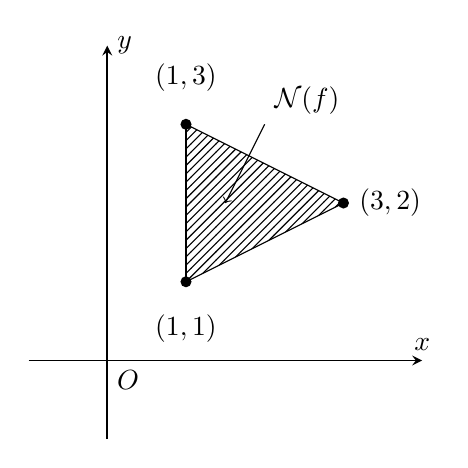
\begin{tikzpicture}
			\label{chapter03:figure:NewtonPolytopeExample}
			% x軸y軸の描画
			\draw[->,>=stealth,semithick] (-1,0)--(4,0)node[above]{$x$};
			\draw[->,>=stealth,semithick] (0,-1)--(0,4)node[right]{$y$};
			% 点の定義
			\coordinate (A) at (1, 1);
			\coordinate (B) at (1, 3);
			\coordinate (C) at (3, 2);
			\coordinate (internal_point) at (1.5, 2);
			\coordinate (explanation_point) at (2, 3);
			% 点の描画
			\draw (0,0) node[below right]{$O$};
			\draw (A) node [below, circle] {$(1, 1)$};
			\draw (B) node [above, circle] {$(1, 3)$};
			\draw (C) node [right, circle] {$(3, 2)$};
			\draw (explanation_point) node [above right] {$\mathcal{N}(f)$};
			\fill (A) circle (2pt) (B) circle (2pt) (C) circle (2pt);
			% 先の描画
			\draw (A)--(B);
			\draw (B)--(C);
			\draw (C)--(A);
			\draw [<-] (internal_point)--(explanation_point);
			% 斜線の描画
			\path [pattern=north east lines] plot [smooth] (A)--(B)--(C);
		\end{tikzpicture}
	\caption{Newton polytope $\mathcal{N}(f)$}
	\end{minipage}
	\begin{minipage}[h]{0.49\columnwidth}
		\centering
		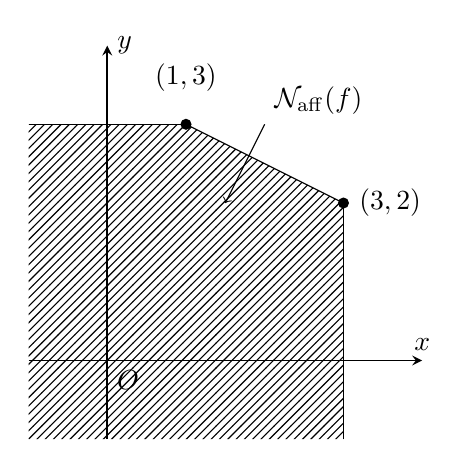
\begin{tikzpicture}
			\label{chapter03:figure:affineNewtonPolyhedronExample}
			% x軸y軸の描画
			\draw[->,>=stealth,semithick] (-1,0)--(4,0)node[above]{$x$};
			\draw[->,>=stealth,semithick] (0,-1)--(0,4)node[right]{$y$};
			% 点の定義
			\coordinate (B) at (1, 3);
			\coordinate (C) at (3, 2);
			\coordinate (D) at (-1, 3);
			\coordinate (E) at (3, -1);
			\coordinate (F) at (-1, -1);
			\coordinate (internal_point) at (1.5, 2);
			\coordinate (explanation_point) at (2, 3);
			% 点の描画
			\draw (0,0) node[below right]{$O$};
			\draw (B) node [above, circle] {$(1, 3)$};
			\draw (C) node [right, circle] {$(3, 2)$};
			\draw (explanation_point) node [above right] {$\mathcal{N}_{\mathrm{aff}}(f)$};
			\fill (B) circle (2pt) (C) circle (2pt);
			% 線の描画
			\draw (B)--(C);
			\draw (D)--(B);
			\draw (C)--(E);
			\draw [<-] (internal_point)--(explanation_point);
			% 斜線の描画
			\path [pattern=north east lines] plot [smooth] (D)--(B)--(C)--(E)--(F);
		\end{tikzpicture}
		\caption{affine Newton polyhedron $\mathcal{N}_{\mathrm{aff}}(f)$}
	\end{minipage}
\end{figure}
図\ref{chapter03:figure:NewtonPolytopeExample}のように,Newton polytopeは単に多項式$f$に含まれる項の指数ベクトルを頂点とした集合となっている.
対して,図\ref{chapter03:figure:NewtonPolytopeExample}のように,affine Newton polyhedronでは,$\mathcal{N}(f)$と$\mathbb{R}^2_{-}$とのMinkowski和を取ることで,"左下"全体を含んだ領域を取る無限集合となっているが,頂点に着目すると,それに伴って"左下"にあった頂点$(1, 1)$がなくなっている.これは,多項式の中で「先頭項になりそうにない次数の低い項」を取り除く操作に対応している.この例では,項$xy$は項順序の定義から先頭項にはならず,affine Newton polyhedronを取ることでそのような項を検出することができることを意味している.

\subsection{\groebner{}基底とNewton polytope}
多項式集合が\groebner{}基底となるためには,Buchbergerアルゴリズムの計算過程にもある通り,全てのSペアが$0$へ簡約される必要がある.その際にS多項式の計算を行うためには,多項式の先頭項を確定させる必要がある.もし,多項式集合における項順序の同値類の数が分かれば,それぞれの適当な代表元において,全てのSペアの簡約が$0$となるかどうかを調べることで,与えられた多項式集合がそのまま\groebner{}基底となるような項順序が存在するのかどうかを確かめることができる.
次の定理では,項順序の同値類を,先程定義した多項式集合のaffine Newton polyhedronで記述するものとなっている.
\begin{theorem}[{\cite[p263, Proposition3.2.1]{gritzmann1993minkowski}}]
	\label{chapter03:theorem:GBD_main_theorem}
	多項式集合$F = \{f_1, \dots, f_k\} \subset K[\bar{X}]$に対して,affine Newton polyhedron $\mathcal{N}_{\mathrm{aff}}(F)$の各頂点は,$F$に関する項順序の同値類と一対一に対応している.
\end{theorem}

\begin{proof}
	多項式$f_i \in F$は$\displaystyle f_i = \sum_{j=1}^{t_i}c_{ij}X^{\alpha_{ij}}$で表されるとする.
	2つの異なる項順序$\bm{w_1}, \bm{w_2} \in \mathbb{R}^n$は多項式集合$F$が任意の$i \in \{1, \dots, k\}$に対して
	$$\max \{(\alpha_{ij}, \bm{w_1}) \; : \; 1 \le j \le t_i\} = \max \{(\alpha_{ij}, \bm{w_2}) \; : \; 1 \le j \le t_i\}$$
	を満たすときに限り等しくなる.
	以下のような項のインデックスに関する集合$\mathcal{J}$を考える.
	$$\mathcal{J} = \{ \bm{j} = (j_1, \dots, j_k) \in \mathbb{N}^k \;:\; \forall i \in \{1, \dots, k\}, \; 1 \le j_i \le t_i\}$$
	$\mathcal{J}$の各要素$\bm{j}$にpolyhedral cone $C_{\bm{j}}$を
	$$C_{\bm{j}} = \{\bm{w} \in \mathbb{R}^n \;:\; \forall i \in \{1, \dots, k\}, \; \forall j \in \{1, \dots, t_i\} \setminus \{j_i\}, \; (\alpha_{ij_i}, \bm{w}) > (\alpha_{ij}, \bm{w}) \}$$
	のように定義する.
	重みベクトル$\bm{w}$が$C_{\bm{j}}$に含まれるのは,$\bm{j}$でインデックス付けされた単項式が$\bm{w}$に関する$F$の先頭項である場合に限られる.したがって,$F$に関する項順序の同値類は、空ではない$C_{\bm{j}}$と一対一に対応している.
	\par
	Newton polytope $\mathcal{N}(F)$は、点$\displaystyle \alpha_{\bm{j}} = \sum^k_{i=1} \alpha_{ij_i}$のconvex hullである(ただし$\bm{j} = (j_1, \dots, j_k) \in \mathcal{J}$).
	また,affine Newton polyhedron $\mathcal{N}_{\mathrm{aff}}(F)$の頂点の集合は,$\mathcal{N}(F)$の頂点の部分集合である.
	頂点$\alpha_{\bm{j}}$は$\mathbb{R}^n$への線型汎関数$(\mathbb{R}_{+}^d \to \mathbb{R}_+)$が最大値である場合に先頭項となるため,その場合に限って$\mathcal{N}_{\mathrm{aff}}(F) (= \mathcal{N}(F) + \mathbb{R}_{-}^n)$の頂点となる.
	これは、$\displaystyle (\alpha_{\bm{j}}, \bm{w}) = \sum_{i = 1}^k \alpha_{j_i}\bm{w}$が他のすべての$\bm{j}^\prime \in \mathcal{J}$に対して$(\alpha_{\bm{j}^\prime}, \bm{w})$より大きいような重みベクトル$\bm{w}$が存在することを意味している.
	しかし,このとき$\bm{w} \in C_{\bm{j}}$となる.よって,空でない$C_{\bm{j}}$はpolyhedron $\mathcal{N}_{\mathrm{aff}}(F)$の頂点への法線円錐(the normal cones to the vertices)であることを示した。
\end{proof}

特に,多項式集合が斉次のとき,次のような系を得られる.
\begin{corollary}[{\cite[p264, Corollary3.2.2]{gritzmann1993minkowski}}]
	\label{chapter03:corollary:GBD_main_corollary}
	斉次な多項式集合$F = \{f_1, \dots, f_k\}$に対して,Newton polytope $\mathcal{N}(F)$の各頂点は,$F$に対する項順序の同値類と一対一対応している.
\end{corollary}
\begin{proof}
	$f_i$が$R_i$-斉次であるとし,$R = R_1 + \cdots + R_k$とする.
	このとき,Newton polytope $\mathcal{N}(F)$はaffine超平面(affine hyperplane)
	$$\left\{ \bm{y} \in \mathbb{R}^n \;:\; \sum_{j=1}^n y_j = R\right\}$$
	に含まれる.
	$\mathcal{N}(F)$のある頂点$\alpha_{\bm{j}}$があるベクトル$\bm{w}$に対して極大(extremal)であるならば,それは任意の$c \in \mathbb{R}_+$に対して$\bm{w} +(c, c, \dots, c)$の方向でも極大(extremal)である.$$(\because \forall \alpha \in \mathcal{N}(F), \; (\alpha, \bm{c}) = cR = (const)\; )$$
	\par
	$c$を適切にとったときに,$\alpha_{\bm{j}}$は$\mathcal{N}_{\mathrm{aff}}(F)$の頂点でもあることを示す.
	$$\beta \in \mathcal{N}_{\mathrm{aff}}(F), \; \gamma \in \mathbb{R}^n_{-}, \; \beta = \alpha + \gamma$$とする.
	$\mathcal{N}_{\mathrm{aff}}(F) \subseteq \mathcal{N}(F)$より,$\beta \in \mathcal{N}(F)$.故に,$(\alpha_{\bm{j}}, \bm{c}) = (\beta, \bm{c}) = cR$.
	よって,
	\begin{align}
		(\bm{w} + \bm{c}, \beta) &= (\bm{w}, \beta) + cR \label{chapter03:formula:GBD_main_corollary_1}\\
		(\bm{w} + \bm{c}, \alpha_{\bm{j}}+\gamma) &= (\bm{w}, \alpha_{\bm{j}}) + cR + (\bm{w}, \gamma) + (\bm{c}, \gamma) \label{chapter03:formula:GBD_main_corollary_2}
	\end{align}
	式(\ref{chapter03:formula:GBD_main_corollary_1})と式(\ref{chapter03:formula:GBD_main_corollary_2})は等しくなるため,
	\begin{equation*}
		(\bm{w}, \gamma) + (\bm{c}, \gamma) = \bm{0}
	\end{equation*}
	よって,
	\begin{align*}
		&\gamma = \bm{0} \\
		\Longleftrightarrow \; & \alpha_{\bm{j}} = \beta \in \mathcal{N}_{\mathrm{aff}}(F)
	\end{align*}
	$\alpha_{\bm{j}} \in \mathcal{N}_{\mathrm{aff}}(F)$がわかったため,定理\ref{chapter03:theorem:GBD_main_theorem}と同様に導ける.
\end{proof}

これらの定理により,\groebner{} basis detectionは次のように解くことができる.多項式集合$F$に対して,
\begin{itemize}
	\item affine Newton polyhedron $\mathcal{N}_{\mathrm{aff}}(F)$を求める.$F$が斉次の場合はNewton polytope $\mathcal{N}(F)$を考える.
	\item その頂点の数をして項順序の同値類の数がわかる.
	\item 適当な代表元において,S多項式のペアが全て$0$に簡約化されるかどうかを調べ,そのような項順序がGBDで求めたいものである.
\end{itemize}
具体的には,定理\ref{chapter03:theorem:GBD_main_theorem}の証明より,次の図のように各頂点を結ぶ辺の法線ベクトルで区切られた領域が,一つの同値類に対応している.
\begin{figure}[h]
	\centering
	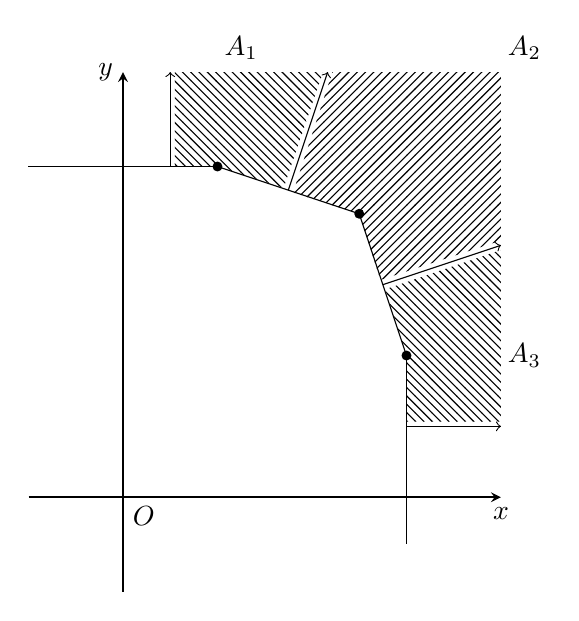
\begin{tikzpicture}[scale=0.6]
		% x軸y軸の描画
		\draw[->,>=stealth,semithick] (-2,0)--(8,0)node[below]{$x$};
		\draw[->,>=stealth,semithick] (0,-2)--(0,9)node[left]{$y$};
		% 点の定義
		\coordinate (A) at (2, 7);
		\coordinate (B) at (5, 6);
		\coordinate (C) at (6, 3);
		\coordinate (A_out) at (-2, 7);
		\coordinate (C_out) at (6, -1);
		\coordinate (x_start) at (1, 7);
		\coordinate (x_end) at (1, 9);
		\coordinate (y_start) at (3.5, 6.5);
		\coordinate (y_end) at (4.33333, 9);
		\coordinate (z_start) at (5.5, 4.5);
		\coordinate (z_end) at (8, 5.3333);
		\coordinate (w_start) at (6, 1.5);
		\coordinate (w_end) at (8, 1.5);
		% 斜線用の点
		\coordinate (x_start_right) at (1.1, 7);
		\coordinate (x_end_right) at (1.1, 9);
		\coordinate (y_start_left) at (3.4, 6.55);
		\coordinate (y_end_left) at (4.23333, 9);
		\coordinate (y_start_right) at (3.6, 6.45);
		\coordinate (y_end_right) at (4.43333, 9);
		\coordinate (z_start_left) at (5.45, 4.6);
		\coordinate (z_end_left) at (8, 5.4333);
		\coordinate (z_start_right) at (5.55, 4.4);
		\coordinate (z_end_right) at (8, 5.2333);
		\coordinate (w_start_left) at (6, 1.6);
		\coordinate (w_end_left) at (8, 1.6);
		% 点の描画
		\draw (0,0) node[below right]{$O$};
		% \draw (A) node [above, circle] {$(1, 3)$};
		% \draw (C) node [right, circle] {$(3, 2)$};
		% \draw (explanation_point) node [above right] {$\mathcal{N}_{\mathrm{aff}}(f)$};
		\fill (A) circle (3pt) (B) circle (3pt) (C) circle (3pt);
		% 線の描画
		\draw (A)--(B);
		\draw (B)--(C);
		\draw (A_out)--(A);
		\draw (C)--(C_out);
		\draw [->] (x_start)--(x_end);
		\draw [->] (y_start)--(y_end);
		\draw [->] (z_start)--(z_end);
		\draw [->] (w_start)--(w_end);
		% 斜線の描画
		% \path [pattern=north east lines] plot [smooth] (D)--(B)--(C)--(E)--(F);
		\path [pattern=north west lines] plot [smooth] (x_end_right)--(x_start_right)--(A)--(y_start_left)--(y_end_left);
		\path [pattern=north east lines] plot [smooth] (y_end_right)--(y_start_right)--(B)--(z_start_left)--(z_end_left)--(8, 9);
		\path [pattern=north west lines] plot [smooth] (z_end_right)--(z_start_right)--(C)--(w_start_left)--(w_end_left);
		% 領域を表す記号の描画
		\draw (2.5, 9.5) node {$A_1$};
		\draw (8.5, 9.5) node {$A_2$};
		\draw (8.5, 3) node {$A_3$};
	\end{tikzpicture}
	\caption{項順序の同値類に対応している領域}
\end{figure}







% 前提とする定義
	% chapter 03
\section{structural \groebner{} basis detection\cite{sturmfels1997structural}}
\groebner{} basis detectionの問題は,結局は項順序の同値類の数だけS多項式の計算をする必要があり,Buchbergerアルゴリズム等の前処理としての役割には適していない.そこで,Buchbergerの判定条件を用いて問題を簡略化したものが問題\ref{chapter03:problem:SGBD}のstructural \groebner{} basis detectionである.
\subsection{$n = k$のとき}
まず,変数の個数$n$と多項式集合の濃度$k$が等しいときを考える.後になってわかることだが,$n \ne k$のときも,この場合のアルゴリズムに帰着して考えることができる.
\par
次のような多項式を例に考える.
\begin{example}
	\label{chapter03:example:example_polynomial_set}
	多項式集合$F = \{f_1, \dots, f_n\}$を$n$変数の多項式環$K[\bar{X}]$の部分集合とし,
	$$f_i = X_{1}^{a_{i1}} + \cdots + X_n^{a_{in}} - 1$$
	と表されるとものとする.
\end{example}
このような多項式集合$F$に対して,項順序$\bm{w} \in \mathbb{R}_{+}^n$における各多項式の先頭項の集合は,
$$\mathrm{HT}_{\bm{w}}(F) = \{X_{\varphi(1)}^{a_{1\varphi(1)}}, \dots, X_{\varphi(i)}^{a_{i\varphi(i)}}\}$$
のように各多項式の先頭項のインデックスを表す写像$\varphi: \{1, \dots, n\} \to \{1, \dots, n\}$によって表すことができる.
SGBDの問題を解くためには,この$\mathrm{HT}_{\bm{w}}(F)$を適切に定める必要があるが,写像$\varphi$で表現可能な$n!$通りの中から探さなくてはならない.
\par
次の補題により,$\mathrm{HT}_{\bm{w}}(F)$は$n!$通りのうち$1$通りに絞られることがわかる.
\begin{lemma}[{\cite[Lemma5]{sturmfels1997structural}}]
	\label{chapter03:lemma:bipartite_graph}
	例\ref{chapter03:example:example_polynomial_set}の条件を満たす多項式集合$F$に対して,
	$$\prod_{i=1}^n a_{i\rho(i)} \ge \prod_{i=1}^n a_{i\varphi(i)}$$
	を満たすような$\rho$は存在しない.
\end{lemma}
\begin{proof}
	$f_i$の項$X_{\varphi(i)}^{a_{i\varphi(i)}}$を先頭項とするような項順序を$\bm{w} = (w_i)_{i \in \{1, \dots, n\}} \in \mathbb{R}_{+}^n$とし,それ以外の任意の像を$\rho \ne \varphi$とする.項順序$\bm{w}$の下で各多項式の先頭項は$X_{\varphi(i)}^{a_{i\varphi(i)}}$となるので,任意の$i \in \{1, 2, \dots, n\}$に対して
	$$w_{\varphi(i)}a_{i\varphi(i)} > w_{\rho(i)}a_{i\rho(i)}$$
	となる.つまり,$\varphi(i) \ne \rho(i)$を満たす$i$が少なくとも$1$つ存在する.
	従って,$n$個の不等式の総積によって,以下の式が得られる.
	\begin{align}
		& \prod_{i=1}^n w_{\varphi(i)}a_{i\varphi(i)} > \prod_{i=1}^n w_{\rho(i)}a_{i\rho(i)} \\
		\Longleftrightarrow & \prod_{i=1}^n w_i a_{i\varphi(i)} > \prod_{i=1}^n w_i a_{i\rho(i)}
	\end{align}
	両辺を$\displaystyle \prod_{i=1}^n w_i > 0$で割ると,
	$$\prod_{i=1}^n a_{i\rho(i)} < \prod_{i=1}^n a_{i\varphi(i)}$$
\end{proof}
この補題により,SGBDを解くために先頭項候補は,総積$\displaystyle \prod_{i=1}^n a_{i\varphi(i)}$
を最大化するような項の組
$$X_{\varphi(1)}^{a_{1\varphi(1)}}, \dots, X_{\varphi(n)}^{a_{n\varphi(n)}}$$
であることがわかる.このような項の組は二部グラフの最大マッチング問題を解くことによって求めることができる(詳細は後述のアルゴリズム\ref{chapter03:algorithm:SGBD}を参照).
\par
次に,実際にそのような項の組$X_{\varphi(1)}^{a_{1\varphi(1)}}, \dots, X_{\varphi(n)}^{a_{n\varphi(n)}}$がそれぞれの先頭項となるような項順序$\bm{w} \in \mathbb{R}_{+}^n$を求める方法を考える.以下の補題により,これは線形計画問題を解くことで求めることができることがわかる.
\begin{lemma}[{\cite[Lemma6]{sturmfels1997structural}}]
	\label{chapter03:lemmma:lin_prog}
	多項式集合$F$を例\ref{chapter03:example:example_polynomial_set}の条件を満たすような集合とし,$X^{\alpha_i}$を多項式$f_i \in F$の項とする.
	任意の$i \in \{1, \dots, n\}$と
	$X^{\beta_i} \ne X^{\alpha_i}$を満たす$f_i$の任意の項$X^{\beta_i}$に対して,指数ベクトルの差のベクトル$\alpha_i - \beta_i$を列として持つ行列を$\varGamma$とする.
	このとき,$\mathrm{HT}_{\bm{w}}(f_i) = X^{\alpha_i}$を満たすような項順序$\bm{w} \in \mathbb{R}_{+}^n$が唯一存在し,連立不等式$\varGamma \bm{w} > 0, \bm{w} > 0$を解くことによって求めることができる.
\end{lemma}
\begin{proof}
	$\mathrm{HT}_{\bm{w}}(f_i) = X^{\alpha_i}$という仮定から,行列$\varGamma$と$\bm{w}$との積は正となる必要がある.
\end{proof}

これらの補題をもとに,$n=k$のときにSGBDを解くアルゴリズムは以下のように記述することができる.
尚,SGBDの条件を満たすような項順序が存在しなかった場合には,ゼロベクトルを返すようにしている.
\begin{algorithm}[htbp]
	\label{chapter03:algorithm:SGBD}
	\caption{solving structural \groebner{} basis detection for $n = k$ {\cite[Algorighm7]{sturmfels1997structural}}}
	\begin{algorithmic}[1]
		\Require 多項式集合$F \subset K[\bar{X}]$
		\Ensure $F$が$\ideal{F}$の\groebner{}基底となるような項順序$w \in \mathbb{R}_{+}^n$ or ゼロベクトル$\bm{0} \in \mathbb{R}^n$
		\For{$1 \le i, j \le n$}
			\If{$X_j^\alpha \notin T(f_i) \quad (\alpha \ne 0)$}
				\State $a_{ij} \gets 0$
			\EndIf
			\State $a_{ij} \gets (f_i\text{の単項式}X_j\text{の最大指数})$
			\If{$X_j^{a_{ij}}X^\alpha \in T(f_i) \quad (\alpha \ne 0)$}
				\State $a_{ij} \gets 0$
			\EndIf
		\EndFor
		\State 頂点が$2n$個ある二部グラフ$B = \{\bar{V}, \bar{E}\}$を次のように構成
		$$\bar{V} = \{u_1, \dots, u_n, v_1, \dots, v_n\}, \quad (u_i, v_i) \in \bar{E} \quad(a_{ij} > 0 \text{のときのみ})$$
		\State $B$の最大マッチング$M$を求める.
		\If{$\left| M \right| < n$}
			\State \Return $\bm{0} \in \mathbb{R}^n$
		\Else 
			\State $M = \{(u_i, v_{\varphi(i)})\;:\; i \in \{1, 2, \dots, n\}\}$
		\EndIf
		\State 行列$\varGamma$を補題\ref{chapter03:lemmma:lin_prog}と同じように構成し,
		$$\begin{cases}
			\varGamma \bm{w} > 0\\
			\bm{w} > 0
		\end{cases}$$
		を解く.
		\State \Return $\bm{w}$
	\end{algorithmic}
\end{algorithm}

\begin{theorem}
	アルゴリズム\ref{chapter03:algorithm:SGBD}は正当性と有限停止性を有する.
\end{theorem}
\begin{proof}
	まず,1行目のfor文において,入力の多項式を例\ref{chapter03:example:example_polynomial_set}の条件を満たすような項のみを残すように変換している.10行目〜16行目は補題\ref{chapter03:lemma:bipartite_graph}に基づいて二部グラフを構成し,17行目では補題\ref{chapter03:lemmma:lin_prog}に基づいて行列を構成し,線形計画問題を解いている.
\end{proof}
このアルゴリズムでは,大きく分けて
\begin{enumerate}
	\item 単項のみから成り,且つ倍単項式が同じ多項式に存在しないような項のみを残す
	\item 二部グラフの最大マッチング問題を解く
	\item 線形計画問題を解く
\end{enumerate}
という$3$つのステップがある.
2つ目のステップでは,Hungarian method\cite{plummer1986matching}にて,3つ目のステップではKhachian's Ellipsoid method\cite{schrijver1998theory}などの方法を採用することで,アルゴリズム全体は多項式時間で解くことができる\cite{sturmfels1997structural}.

\subsection{$n \ne k$のとき}




















% Groebner基底とNewton polytope
	% chapter 03
\section{\groebner{}基底の構造的な検出}
\groebner{} basis detectionの問題は,結局は項順序の同値類の数だけS多項式の計算をする必要があり,Buchbergerアルゴリズム等の前処理としての役割には適していない.そこで,Buchbergerの判定条件を用いて問題を簡略化したものが問題\ref{chapter03:problem:SGBD}のstructural \groebner{} basis detectionである.
まずは次のような多項式を例に考える.
\begin{example}
	多項式集後$F = \{f_1, \dots, f_n\}$を$n$変数の多項式環$K[\bar{X}]$の部分集合とし,
	$$f_i = X_{1}^{a_{i1}} + \cdots + X_n^{a_{in}} - 1$$
	と表されるとものとする.
\end{example}
この多項式集合$F$に対して,項順序$\bm{w} \in \mathbb{R}_{+}^n$における各多項式の先頭項の集合は,$\mathrm{HT}_{\bm{w}}(F) = \{X_{\varphi(1)}^{a_{1\varphi(1)}}, \dots, X_{\varphi(i)}^{a_{i\varphi(i)}}\}$% Groebner基底の構造的な検出

	% ------chapter04
	\chapter{パラメータを伴った場合への拡張}\label{chapter04:chapter_num}

	% ------chapter05
	\chapter{パラメータ空間の分割の効率化}\label{chapter05:chapter_num}


	% ------reference
	\bibliographystyle{alpha}% [apalike] or [alpha]
	\bibliography{bibliography}

\end{document}